\section{Network Layer}
\paragraph{Schicht 3: Internet}

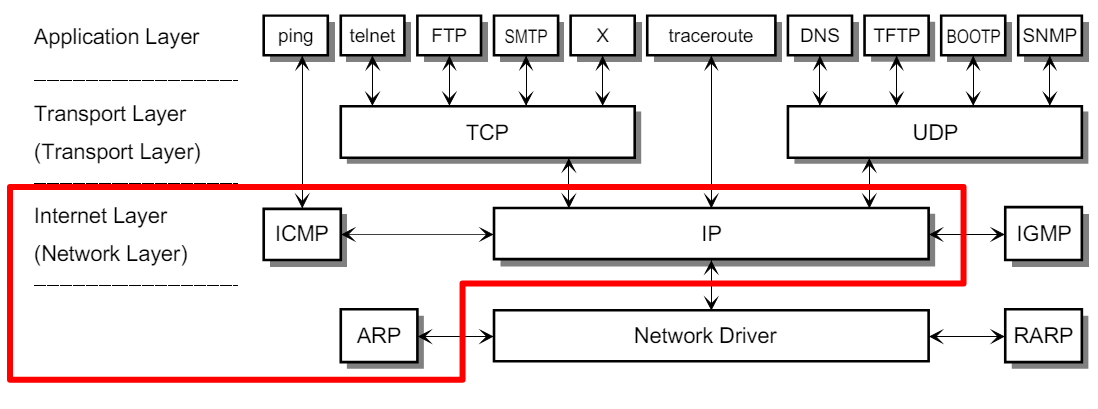
\includegraphics[width=1\linewidth]{images/orientierung_network_layer.png}

\begin{definition}{Die Netzwerkschicht}\\
    NUR Transport der IP-Pakete $\rightarrow$ höhere Layer übernehmen:
        \begin{itemize}
            \item Fehlerfreie, komplette Übertragung
            \item Richtige Reihenfolge, Flusskontrolle
        \end{itemize}
\end{definition}

\begin{lemma}{Grundsätze des Internets}
    \begin{itemize}
        \item Jedes Netzwerk soll für sich selbst funktionsfähig sein
        \item Die Kommunikation basiert auf «best effort»
        \item Die Verbindung der Netze erfolgt durch Black Boxes
        \item Keine zentrale Funktionssteuerung wird benötigt
    \end{itemize}
\end{lemma}

\begin{definition}{Kommunikationsobjekte} OSI Layern zugeordnet
       \begin{itemize}
        \item \textcolor{orange}{(Application-)Message/Stream} Layer 5-7
        \item \textcolor{green}{(Transport-)Paket, Datagram} Layer 4
        \item \textcolor{blue}{(IP-)Paket (früher Datagram)} Layer 3
        \item \textcolor{pink}{(HW-specific) Frame} Layer 1-2
    \end{itemize}
\end{definition}



\subsection{Netzwerk Applikationen und Protokolle}

\subsubsection{Routing}

\begin{definition}{Router} verbinden Subnetze (Ethernet, xDSL, WLAN, etc.)
    \begin{itemize}
        \item empfangen nur Pakete, die direkt an sie adressiert sind
        \item Weiterleitung erfolgt anhand der Network Layer Adresse
        \item Benutzen immer den optimalen Pfad.
    \end{itemize}
\end{definition}
    

\begin{concept}{Routing and Forwarding}
    \begin{itemize}
        \item Routing: Aufbau und Update der Routingtabellen in den Knoten
            \begin{itemize}
                \item Router müssen optimalen Pfad zu jedem Host kennen
                \item kleine oder Teilnetze: Statische Konfiguration
                \item grössere Netze: Dynamisch durch Routing-Protokolle: Topologie des Netzes ermitteln $\rightarrow$ ideale Pfade bestimmen
            \end{itemize}
        \item Forwarding: Weiterleiten der Daten
        \begin{itemize}
            \item Aufgrund von Routingtabellen Datenpakete weiterleiten
        \end{itemize}
    \end{itemize}
\end{concept}

\begin{definition}{Routing-Tabelle} Info wie jedes Netz/Interface erreicht werden kann
    
    \begin{itemize}
        \item Für Weiterleitungsentscheidung notwendige Informationen:
        \begin{itemize}
            \item Eintrag für jedes erreichbare Netz (Netzadresse, Netzmaske)
            \item Interfaces, über die die Netze erreicht werden können
            \item IP-Adresse des nächsten Routers, wenn Zielnetz nicht direkt erreicht werden kann
        \end{itemize}
        \item Eigenschaften:
        \begin{itemize}
            \item sortiert nach Länge der Netzmaske, von oben nach unten durchsucht
            \item erster Eintrag der passt wird verwendet, default Eintrag am Schluss passt immer
        \end{itemize}        
    \end{itemize}
\end{definition}

\subsubsection{IPv4}

\begin{KR}{IP-Header Format}
    Ein IP-Packet besteht aus einem Header (min. 20 Byte) und Nutzdaten.
    \begin{itemize}
        \item \textcolor{blue}{Version} IPv4 / IPv6
        \item \textcolor{blue}{IHL} Header Length in 4-Byte (20 Byte → IHL = 5)
        \item \textcolor{blue}{Type of Service} neu Differentiated Services (DS), Erlaubt Priorisierung, Einteilung der Daten in Verkehrsklassen
        \begin{itemize}
            \item DSCP: spez. Verhalten bzgl. Weiterleitung
            \item ECN: kann drohende Überlast markieren
        \end{itemize}
        \item \textcolor{blue}{Total Length} Länge des IP-Packets (Header + Nutzdaten)
        \item \textcolor{Goldenrod}{ID Number} Identifikation des IP-Pakets / Fragmente, erlaubt Identifikation zusammengehöriger Fragmente
        \item \textcolor{Goldenrod}{Flags} Kontroll-Flags für Fragmentierung (0/DF/MF)
        \item \textcolor{Goldenrod}{Fragment Offset} Gibt an, wo ein Fragment hingehört
        \item \textcolor{green}{Time to Live} anz. Sek, Hop-Counter, 0 → Paket wird verworfen
        \item \textcolor{green}{Protocol} Übergeordnetes Protokoll
        \item \textcolor{purple}{Header Checksum} verhindert fehlgeleitete Pakete ($\times $ Nutzdaten)
        \item \textcolor{purple}{Source Address} Wer das Paket ursprünglich abgesendet hat
        \item \textcolor{purple}{Destination Address} Wer das Paket schliesslich erhalten soll
        \item \textcolor{purple}{Options/Padding} variabel, füllt auf ein Vielfaches von 32Bits auf
    \end{itemize}
        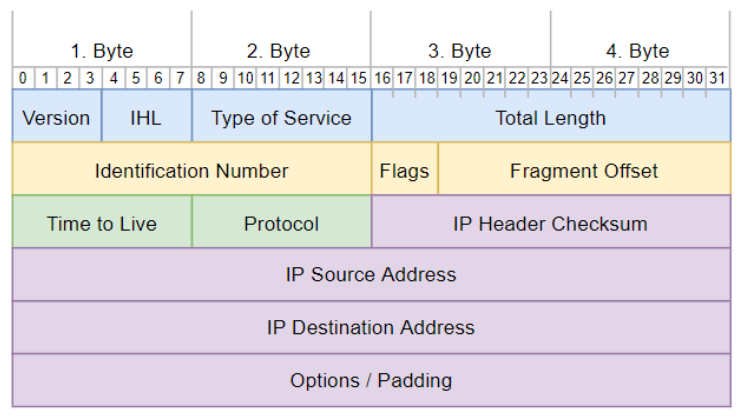
\includegraphics[width=1\linewidth]{images/internet_protokoll_format_ip.png}\\
    Das unterliegende Netz limitiert die Grösse eines Pakets (Maximum Transfer Unit). Der Sender kennt die MTU der Netze nicht.\\
\end{KR}

\begin{definition}{Fragmentierung}
    \begin{itemize}
        \item Länge der Nutzdaten = Vielfaches von 8 Bytes
        \item Die Pakete haben die gleiche und grösstmögliche Länge
        \item Identification Number, Flags und Fragment Offset (siehe \textcolor{Goldenrod}{gelbe Felder} in Grafik oben) wichtig für Fragmentierung
        \item früher von Router durchgeführt, heute im Sender
    \end{itemize}
\end{definition}

\begin{formula}{Reassembly}
    nutze Flags (0/DF/MF) und Fragment Offset
    \begin{itemize}
        \item Zusammensetzen beim Zielhost
        \item Letztes Fragment: MF = 0
    \end{itemize}
        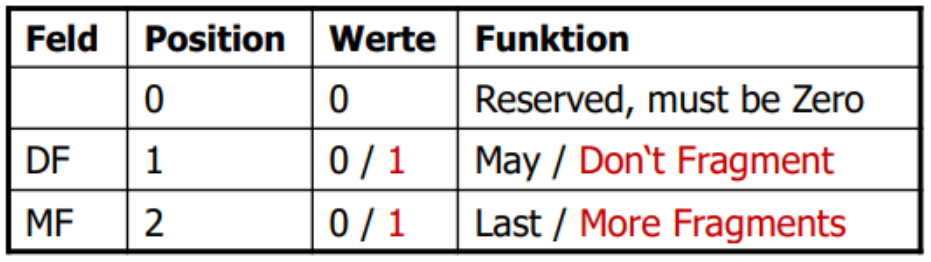
\includegraphics[width=0.75\linewidth]{images/reassembly.png}\\
        Kombination mit DF und MF erlaubt vollständige Rekonstruktion ohne explizite Übertragung der ursprünglichen Paketgrösse
\end{formula}

\subsubsection{Internet Protokolle (IP)}

\begin{definition}{Hierarchische Adressierung}\\
IP-Adressen sind zweistufig hierarchisch
\begin{itemize}
    \item IP-Adresse eines Hosts = Netzadresse + Interface-Adresse
\end{itemize}
\end{definition}

\begin{definition}{Terminologie}
    \begin{itemize}
        \item Sender und Empfänger $\rightarrow$ Hosts
        \item IP bietet einen unzuverlässigen, verbindungslosen Dienst
        \begin{itemize}
            \item IP-Adr. identifiziert Host-Interface (nicht den Host) eindeutig innerhalb des Netzwerks
            \item Jeder Host hat min. eine Adresse, Multi-Homed Hosts mehrere
        \end{itemize}
    \end{itemize}
\end{definition}

\begin{formula}{Netzadresse}
    \begin{itemize}
        \item Reserviert: Darf nicht für Interfaces verwendet werden!
        \item Tiefste Adresse im Subnetz (Interface-Adressbits alle 0)
        \item Berechnet durch: Interface-Adresse AND Subnetzmaske
    \end{itemize}
\end{formula}

\begin{formula}{Broadcast-Adresse}
    \begin{itemize}
        \item Reserviert: adressiert alle Interfaces in einem Subnetze
        \item Höchste Adresse im Subnetz (All Ones Broadcast)
        \item Berechnet durch: Interface-Adresse OR Invertierte Subnetzmaske
    \end{itemize}
\end{formula}

\begin{concept}{Subnetzmaske}\\
    bestimmt die Grenze zwischen Netz- und Interface-Adressbits:\\
        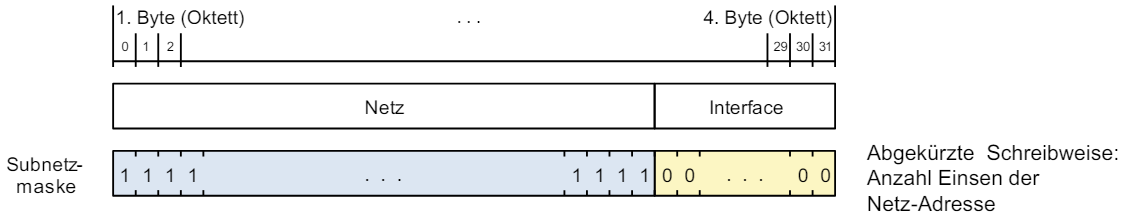
\includegraphics[width=1\linewidth]{images/subnetzmaske.png}\\
    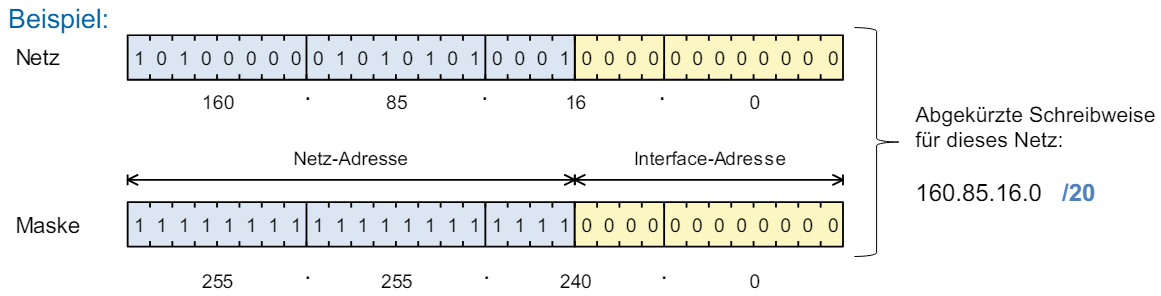
\includegraphics[width=1\linewidth]{images/subnetzmaske_bsp.png}   
\end{concept}

\begin{formula}{Netzmasken}\\
    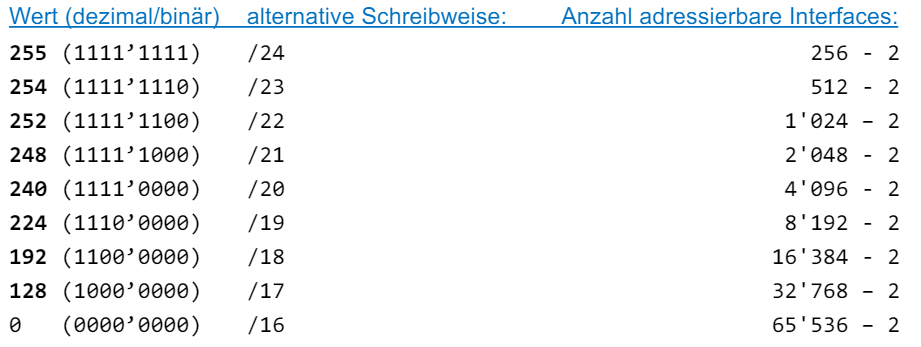
\includegraphics[width=1\linewidth]{images/subnetzmaske_bsp_2.png}
\end{formula}

\begin{KR}{Rechnen mit Netzmasken}\\
    Typische Internet-Adressen Aufgabenstellung: Berechnen Sie die fehlenden Informationen\\
        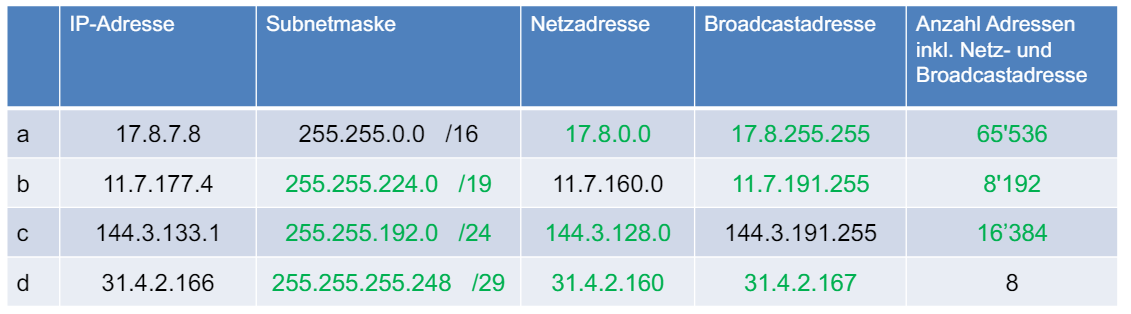
\includegraphics[width=1\linewidth]{images/rechenne_mit_netzmasken.png}
\end{KR}

\subsubsection{Flaches und Hierarchisches Routing}

\begin{concept}{Flaches Routing}
    \begin{itemize}
        \item Router kennt (evtl. mehrere) explizite Wege zu jedem Zielnetz
        \begin{itemize}
            \item Pakete an unbekannte Netze werden verworfen
        \end{itemize}
        \item Einsatz: stark vermaschte Netzen oder im zentraler Bereich (Backbone)
        \item Nachteil: Sehr grosse Routing-Tabellen
    \end{itemize}
\end{concept}

\begin{example2}{Flaches Routing Übung}\\
Was geschieht mit dem IP-Paket?
    \begin{itemize}
        \item Kein Unterbruch?\\ Es wird nach gemäss dem 4. Eintrag der Routingtabelle von Router B an p0 weitergeleitet
        \item Unterbruch von p0 / Router B ? \\ Es wird gemäss Eintrag 5 in der Routingtabelle von Router B an p2 weitergeleitet.
        \item zusätzlicher Unterbruch p0 / Router C ?\\ Router C kann das IP-Paket nicht weiterleiten, es IP-Paket erreicht den Empfänger nicht.
    \end{itemize}
        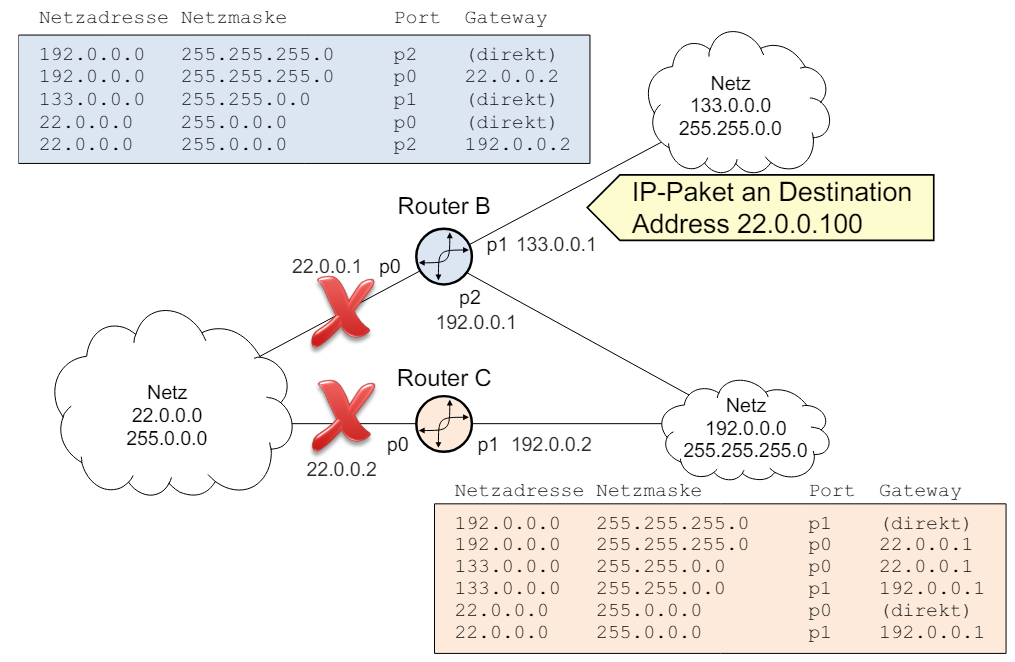
\includegraphics[width=1\linewidth]{images/flaches_routing_bsp.png}
\end{example2}

\begin{concept}{Hierarchisches Routing (Default)}
    \begin{itemize}
        \item Router kennt die direkt angeschlossenen Netze seiner Interfaces und genau einen anderen Router, an den er alles schickt, was für andere Netze bestimmt ist
        \begin{itemize}
            \item Der nächste Router geht genau gleich vor
        \end{itemize}
        \item Einsatz am „Rand“ von Netzen Hosts, ccess Router
        \item Kleine Routing-Tabellen mit jeweils einem Default-Eintrag
    \end{itemize}
        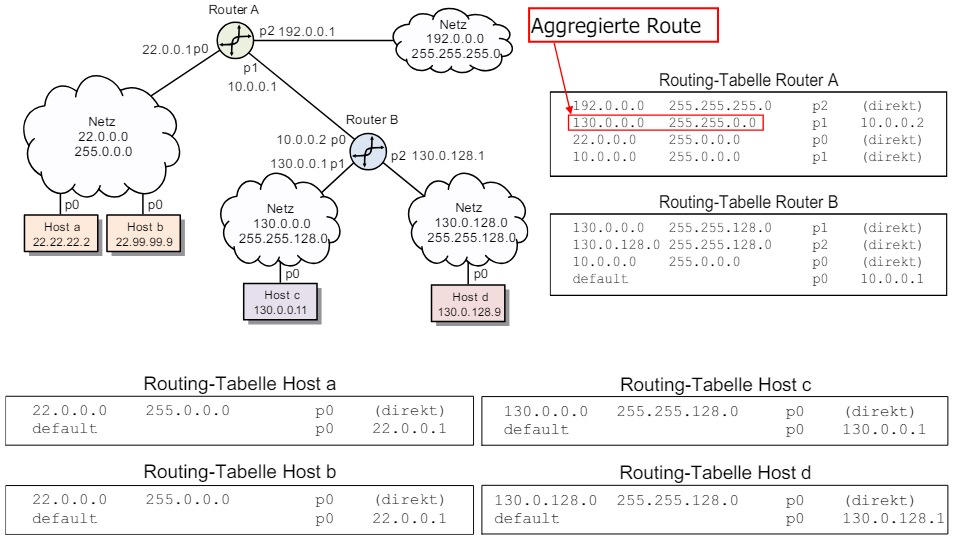
\includegraphics[width=1\linewidth]{images/hierarchisches_routing.png}
\end{concept}

\subsubsection{Classful Routing: Sub-/Supernetting}

\begin{concept}{Classful Routing}\\
    Ursprünglich war der IP Adressbereich in fünf Netzklassen (A - E) eingeteilt
    \begin{itemize}
        \item Eine Prefix (die ersten 4 Adress-Bits) erlaubt die Bestimmung der Klasse
    \end{itemize}
        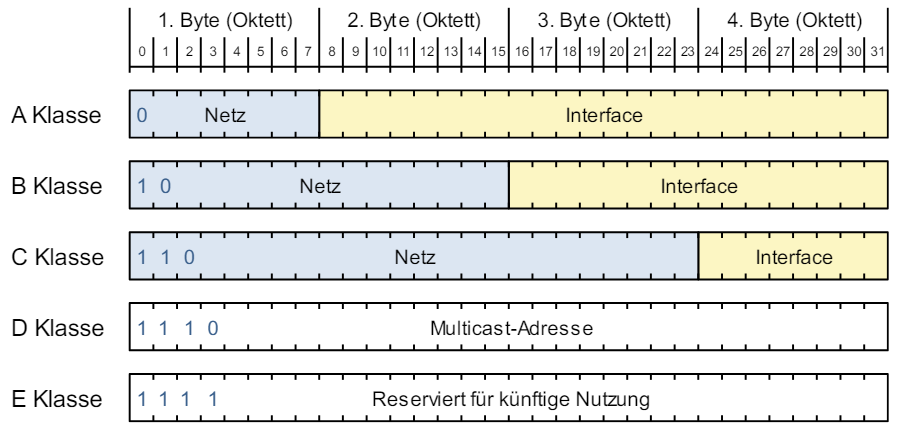
\includegraphics[width=1\linewidth]{images/classfulrouitng.png}
\end{concept}

\begin{example2}{Classful Routing}\\
    Beispiel von 4 zusammengeschlossenen Netzen:\\
        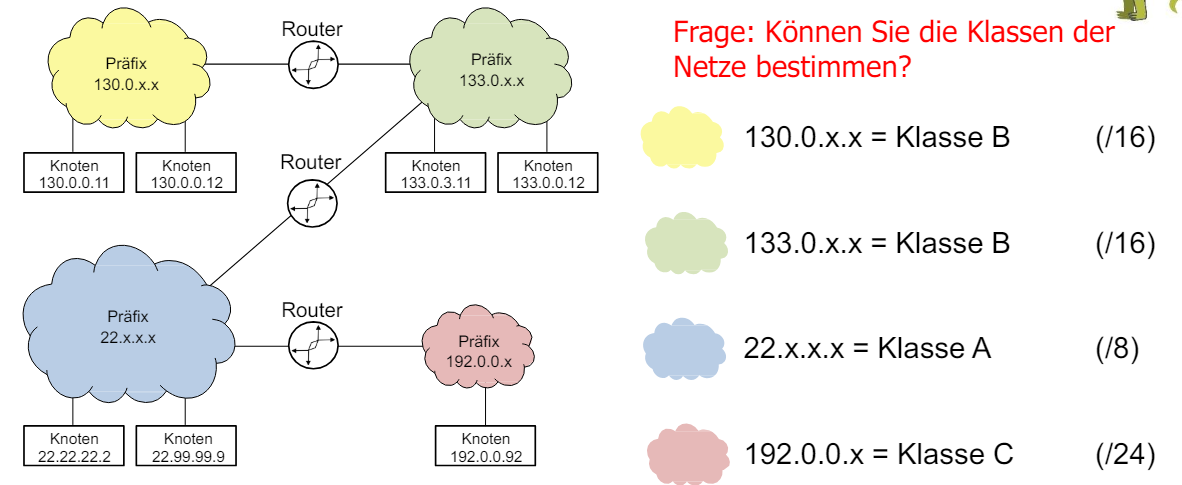
\includegraphics[width=1\linewidth]{images/classful_routing.png}
\end{example2}

\begin{KR}{Internet-Adressierung (IPv4 Netz-Klassen)}\\
    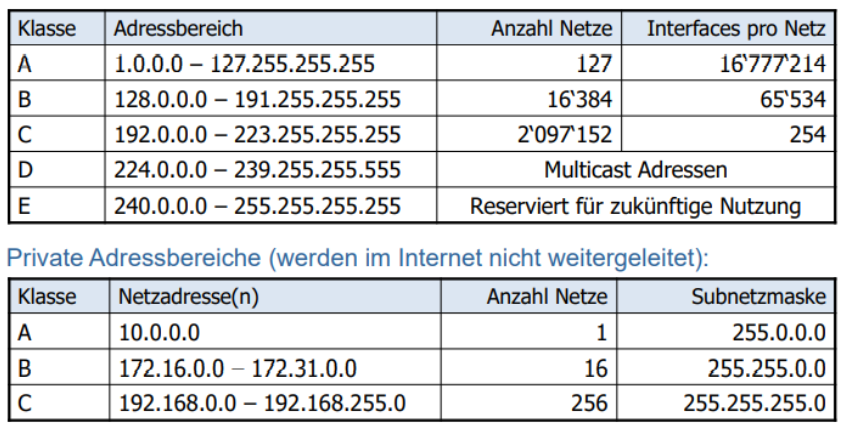
\includegraphics[width=0.9\linewidth]{images/ipv4.png}
\end{KR}

\begin{formula}{Adressbereiche für Classful Routing}
    \begin{itemize}
        \item Die klassischen Netze fixer Grösse sind unflexibel
        \begin{itemize}
            \item Klasse C Netze sind für Unternehmen zu klein
            \item Klasse A Netze sind zu gross
            \item Klasse B Netze sind zu wenig
        \end{itemize}
        \item Abhilfe schafft CIDR – Classless Inter-Domain Routing
        \begin{itemize}
            \item Flexible Verwendung von Netzmasken beliebiger Länge
            \item Aufteilung grosser Netze in kleinere Subnetze, Zusammenfassen mehrerer kleiner Netze zu einem gemeinsamen grösseren Netz
        \end{itemize}
    \end{itemize}
\end{formula}

\begin{definition}{localhost}\\
    Loopback-Adressen
    \begin{itemize}
        \item Das gesamte A-Netz 127.0.0.0/8 ist für Loopback-Test reserviert
        \item Daten werden an ein emuliertes Loopback-Gerät geschickt, das sie direkt zurück gibt (kein Netzwerk/-Interface nötig).
    \end{itemize}
\end{definition}

\subsubsection*{Sub- und Supernetting}

\begin{concept}{Supernetting}
    Zusammenfügen von kleinen Netzen\\
    Hintereinanderliegende Class C Netze können zu einem Netz zusammengefügt werden. \\
    Kann ebenfalls helfen, Routingtabellen in Routern zu verkleinern (Aggregate Routes)
\end{concept}

\begin{example}
    Beispiel: Zusammenfassen von 4 Class C Netzen (22 = 2 Bits der Subnetzmaske)\\
        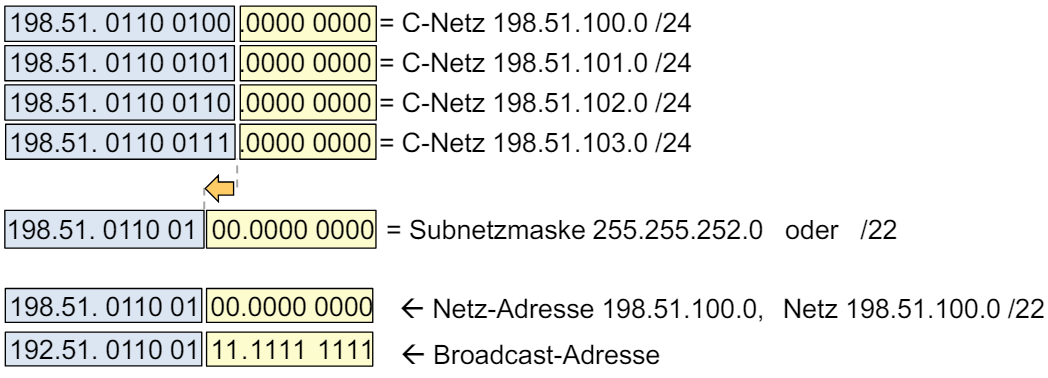
\includegraphics[width=1\linewidth]{images/example_supernetting.png}
\end{example}

\begin{concept}{Subnetting}
    Aufteilung in kleinere Netze\\
    Die ZHAW besitzt das Klasse B Netz 160.85.0.0
    \begin{itemize}
        \item Total $2^{16} \cong 65000$  Hosts
        \item Die ZHAW möchte dieses in 8 kleinere Subnetze aufteilen → Subnetting
    \end{itemize}
    Verschieben der Netzmasken-Bits: $8 = 2^3$, es werden 3 1en in der binären Netzmaske ergänzt
    \begin{itemize}
        \item 3 Bits identifizieren 8 Subnetze (000 → 111)
        \item Die Netzmaske verändert sich von /16 zu /19 (255.255.0.0 → 255.255.224.0)
        \item Der Interface-Anteil verändert sich von $2^{16}$ zu $2^{13}$ = 8192 IP Adressen pro Subnetz
    \end{itemize}
        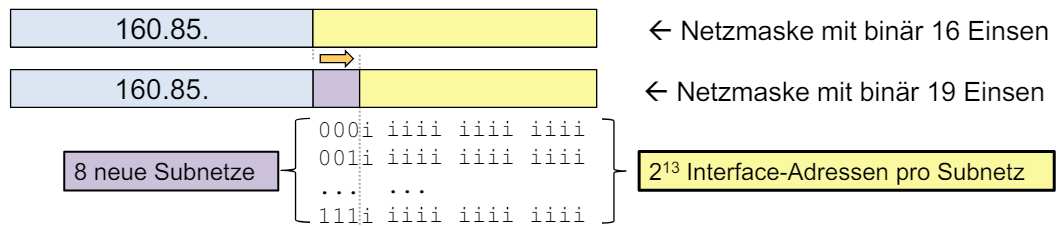
\includegraphics[width=1\linewidth]{images/subnetting1.png}\\
    Damit haben wir 8 neue Subnetze mit den folgenden Netzadressen:\\
        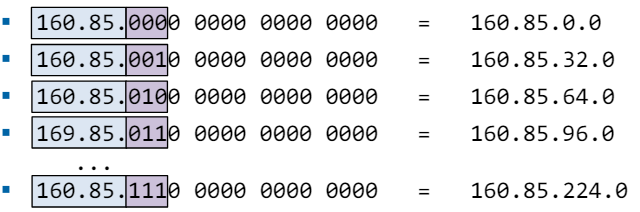
\includegraphics[width=0.75\linewidth]{images/subnetting2.png}
    \begin{itemize}
        \item Der Netz-Anteil der binären Netzmaske hat nun 19 statt 16 "1" → Subnetzmaske: 255.255.224.0 oder /19
        \item Der Host-Anteil der binären Nutzmaske hat nun 13 statt 16 "0" → Anzahl Hostadressen 8'192
    \end{itemize}
    Das zweite Netz oben wird deshalb korrekt wie folgt gekennzeichnet:
    \begin{itemize}
        \item 160.85.32.0 / 255.255.224.0 oder 160.85.32.0 /19
    \end{itemize}
    Das fünfte Netz wird wie folgt gekennzeichnet:
    \begin{itemize}
        \item 160.85.128.0 / 255.255.224.0 oder 160.85.128.0 /19
    \end{itemize}
    \textcolor{pink}{Wichtige Regel: Eine Netzwerkadresse ist immer ein Vielfaches der Netzgrösse!}
\end{concept}

\begin{example2}{Flexible Aufteilung eines Netzbereiches}\\
    Ein KMU mit 4 Standorten hat von seinem ISP das Netz 193.72.32.0 /21 erhalten. Das KMU hat 3 grössere und einen kleineren Standort und will diese redundant verbinden.\\
        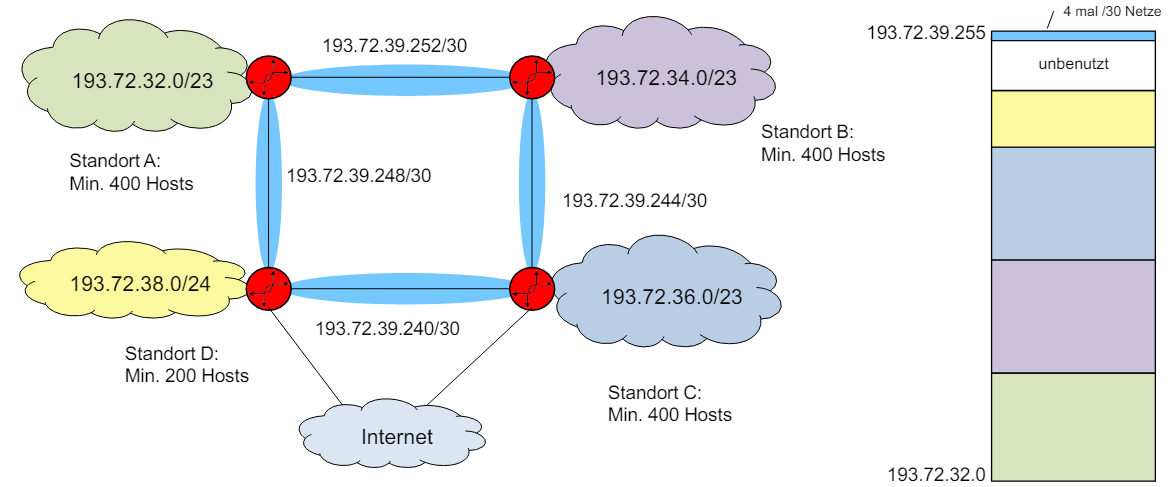
\includegraphics[width=1\linewidth]{images/flexible_aufteilung_netzbereich.png}    
\end{example2}



\subsubsection{IPv6}

\begin{definition}{IPv6}
    \begin{itemize}
        \item IPv6 ist in RFC 2460 spezifiziert
        \item 128-bit Adressen; diese werden mit je zwei-Bytes in Hex-Darstellung notiert und durch Doppelpunkte getrennt
        \item IPv6 verwendet Extension Headers, um den Basic Header zu vereinfachen
        \item Ein Interface kann mehr als eine IPv6 Adresse haben
        \begin{itemize}
            \item Ein Interface hat in der Regel eine lokale und zwei globale IPv6 Adressen:
            \item Eine MAC-basierte und eine nicht von der Hardware abhängige.
        \end{itemize}
        \item verwendet zur Abfrage der Layer-2 Adressen NDP statt ARP
        \item Domain Name Service (DNS)
        \begin{itemize}
            \item IPv4 stellt an den Resolver Anfragen nach A-Records
            \item IPv6 stellt an den Resolver Anfragen nach AAAA-Records
        \end{itemize}
        \item hat sich nicht durchgesetzt weil:
        \begin{itemize}
            \item nicht so einfach lesbar wie IPv4
            \item Viele Probleme von IPv4 konnten gelöst werden
            \item IPv6 ist nicht rückwärtskompatibel
        \end{itemize}
    \end{itemize}
    
\end{definition}

\begin{KR}{Key Takes}
    \begin{itemize}
        \item Der IP-Header besteht aus 20 Bytes (ohne Optionen)
        \item Um über Netze mit verschiedenen Maximum Transfer Units (MTU) arbeiten zu können, unterstützt IP Fragmentierung und Reassembly
        \begin{itemize}
            \item Heute wird in der Regel beim Sender fragmentiert und im Ziel-Host reassembliert
            \item Path MTU discovery mittels ICMP kann verwendet werden, um die kleinste MTU auf dem Weg zum Ziel-Host zu identifizieren
        \end{itemize}
        \item IP-Pakete werden in Ethernet Frames gekapselt und von jedem Router wieder ausgepackt und erneut gekapselt.
        \begin{itemize}
            \item Dazu muss der Router die Layer-2 Adresse (MAC-Adresse) des nächsten Routers/Hosts kennen (ARP-Cache) oder erfragen (ARP-Request)
        \end{itemize}
        \item ICMP wird verwendet, um Fehler innerhalb der Netzwerkschicht zu behandeln (keine Retransmissions)
        \begin{itemize}
            \item ICMP-Nachrichten werden in IP-Pakete gekapselt, werden aber dennoch der NetzwerkSchicht zugeordnet
        \end{itemize}
    \end{itemize}
\end{KR}

\columnbreak

\subsection{Kapselung und Adressauflösung}

\begin{definition}{Kapselung eines IP-Pakets im Ethernet Frame}\\
    Meist wird heute Ethernet-Encapsulation verwendet
    \begin{itemize}
        \item Das IP-Paket wird direkt im Nutzdatenteil des Frames übertragen
        \item Das Type Feld des Ethernet Frames erhält den Wert 0800 (hex)
        \item Die MTU ist damit 1500 Bytes
    \end{itemize}
        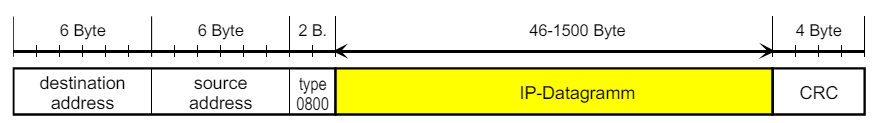
\includegraphics[width=1\linewidth]{images/kapselung_ip_paket.png}
\end{definition}

\begin{KR}{Kapselung und Adressauflösung}\\
    ARP (Address Resolution Protocol)
    \begin{itemize}
        \item Ermittelt HW-Adresse (MAC) zu einer IP-Adresse
    \end{itemize}
    Internet Control Message Protocol (ICMP)
    \begin{itemize}
        \item Übertragungen von Fehlermeldungen oder Informationsaustausch
    \end{itemize}
\end{KR}

\begin{example2}{Übertragung eines IP-Pakets mit Encapsulation}\\
    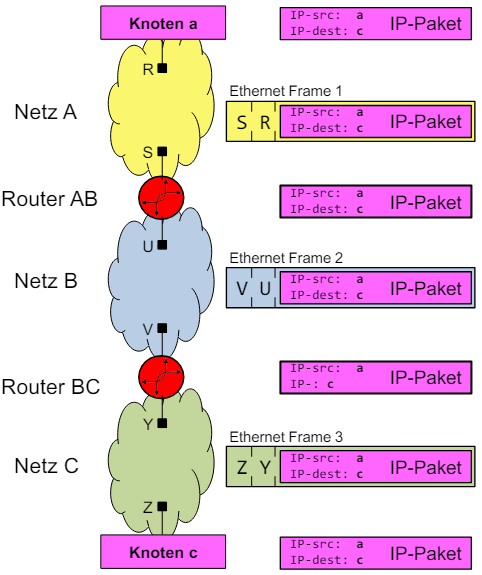
\includegraphics[width=0.6\linewidth]{images/encapsulation_bsp.png}\\
    Was geschieht bei der Übertragung genau?
    \begin{itemize}
        \item Knoten a sendet ein IP-Paket an Knoten c
        \begin{itemize}
            \item das Paket enthält die IP-Adressen von a und c
        \end{itemize}
        \item Knoten a konsultiert die Routing Tabelle und sieht:
        \begin{itemize}
            \item dass c über den Router AB erreicht werden kann, und
            \item Kennt nun die IP-Adresse von Router AB
        \end{itemize}
        \item Knoten a generiert ein Ethernet Frame, welches an die Hardware-adresse S von Router AB gesendet wird
        \begin{itemize}
            \item a muss aus der IP-Adresse von Router AB die Hardware-Adresse S herausfinden
            \item \textbf{Adressauflösung}
        \end{itemize}
        \item Router AB empfängt das Ethernet Frame, packt das IP-Paket aus und modifiziert den Header (TTL)
        \item Router AB konsultiert die Routing Tabelle und sieht:
        \begin{itemize}
            \item dass c über den Router BC erreicht werden kann, und
            \item Kennt nun die IP-Adresse von Router BC
        \end{itemize}
    \end{itemize}
    \textcolor{pink}{Die IP-Adressen a und c bleiben während der gesamten Übertragung unverändert}\\
\end{example2}

\subsubsection*{Address Resolution Protocol (ARP)}

\begin{concept}{ARP}
    Grundprinzip von ARP
    \begin{itemize}
        \item Ermittlung der Hardwareadresse (MAC) zu einer IP-Adresse
        \item ARP-Request wird an Broadcast-Adresse gesendet
        \item ARP-Response wird von Knoten mit angefragter IP-Adresse an Absender gesendet
        \item Die ARP-Tabelle speichert bekannte <IP-MAC> Kombinationen für eine gewisse Zeit
    \end{itemize}
        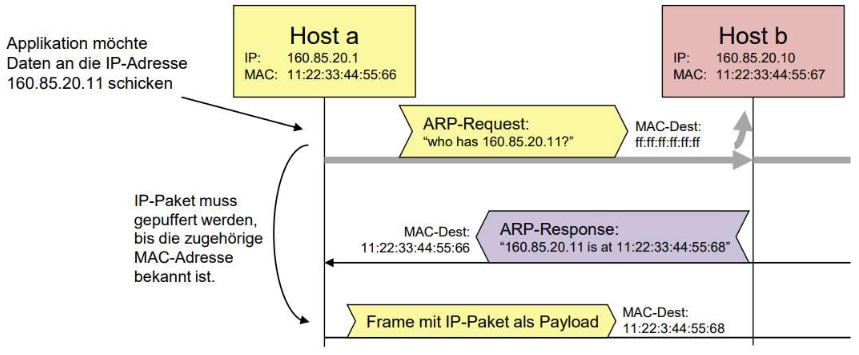
\includegraphics[width=1\linewidth]{images/arp_concept.png}
\end{concept}

\begin{formula}{ARP Nachrichtenstruktur}\\
    ARP-Request und ARP-Response sind je in genau einem Ethernet Frame enthalten mit Type x0806
    \begin{itemize}
        \item Beim Request ist die Destination Address FF-FF-FF-FF-FF-FF (Broadcast Frame) und die Hardware Address of Target ist 0
    \end{itemize}
        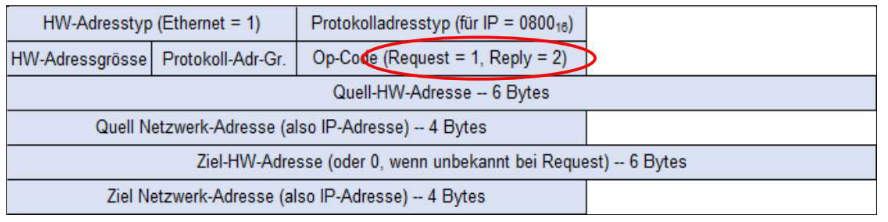
\includegraphics[width=1\linewidth]{images/arp_nachrichtenstruktur.png}
\end{formula}

\begin{KR}{ARP Implementierung und Verwendung}
    \begin{itemize}
        \item Ein ARP-Request/Response für jedes IP-Paket wäre sehr ineffizient
        \begin{itemize}
            \item Jeder Knoten führt eine Tabelle (ARP-Cache) mit bekannten HW-Adressen
        \end{itemize}
        \item Aufgelöste (bekannte) Mappings IP Adresse $\rightarrow$ Hardwareadresse werden im ARP-Cache für gespeichert
        \begin{itemize}
            \item Erneuerung nach Ablauf eines Timers, typisch: einige Minuten
        \end{itemize}
        \item Abfrage/Modifizieren des ARP-Cache mit arp (Windows):
        \begin{itemize}
            \item arp -a: Anzeigen aller Einträge
            \item arp -d ip\_addr: Löschen eines Eintrags
            \item arp –s ip\_addr hw\_addr: Setzen eines Eintrags
        \end{itemize}
        \item Neue / empfohlene Befehle für Linux:
        \begin{itemize}
            \item ip neigh \{ add | del | show\}
        \end{itemize}
    \end{itemize}
    Weitere Verwendung:
    \begin{itemize}
        \item Erkennung von Adresskonflikten
        \begin{itemize}
            \item Nach einer Adresszuweisung (manuell oder per DHCP) wird ein ARP-Request an die eigene IPAdresse gerichtet, um zu prüfen, ob kein anderer Host im LAN die Adresse verwendet
            \item Falls eine Antwort kommt, liegt ein Adresskonflikt vor
        \end{itemize}
        \item Erneuerung von Einträgen im ARP-cache
        \begin{itemize}
            \item Linux Systeme senden in diesem Fall einen ARP-Request als Unicast
            \item Reduziert Broadcast-Last im Netz
        \end{itemize}
    \end{itemize}
\end{KR}



\subsubsection{Internet Control Message Protocol (ICMP)}

\begin{concept}{Internet Control Message Protocol (ICMP)}\\
    Übertragung von Fehlermeldungen oder Informationsaustausch auf Internet Layer, z.B.
    \begin{itemize}
        \item Time to live (TTL) hat den Wert 0 erreicht
        \item Ein Host möchte testen, ob ein anderer Host „up“ ist ICMP Meldungen werden in IP Paketen gekapselt
        \item Sieht aus wie ein Protokoll eines höheren Layers, welches den Internet Layer verwendet
        \item ICMP ist aber so eng mit IP verbunden, dass es zum Network Layer gezählt wird
    \end{itemize}
        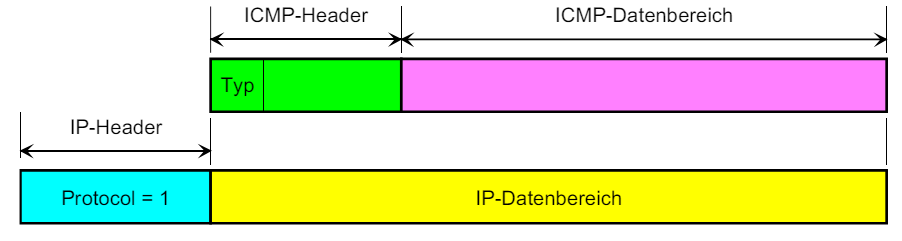
\includegraphics[width=0.75\linewidth]{images/icmp.png}
\end{concept}

\begin{KR}{ICMP Format}\\
    Header:
    \begin{itemize}
        \item \textcolor{blue}{Type} ICMP Typ
        \item \textcolor{green}{Code} Message Details
        \item \textcolor{green}{Checksum} Prüfsumme über die ICMP Meldung
        \item \textcolor{pink}{depends on code} Unterschiedliche Werte und Verwendung je nach ICMP Typ
    \end{itemize}
    \textcolor{purple}{Datenbereich} IP-Header und 64 Bits of Original Datagram
    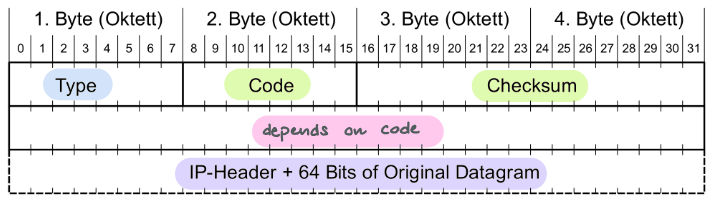
\includegraphics[width=1\linewidth]{images/icmp_details.png}
\end{KR}

\begin{formula}{ICMP Meldungstypen}
    \begin{itemize}
        \item ICMP benutzt direkt IP - keine Garantie, dass die Meldungen je ankommen
        \item Meldungen sind NUR informativ gedacht
    \end{itemize}
    \begin{center}
        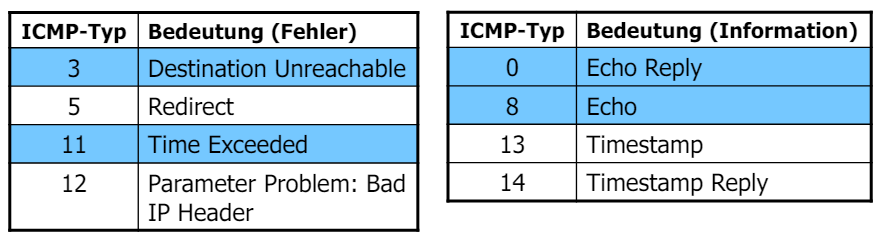
\includegraphics[width=0.8\linewidth]{images/icmp_medlungstypen.png}
    \end{center}
    Codes:
    \begin{itemize}
        \item 0 = net unreachable (Router)
        \item 1 = host unreachable (Router)
        \item 2 = protocol unreachable (Ziel Host)
        \item 3 = port unreachable (Ziel Host)
        \item 4 = fragmentation needed and DF set (Router)
        \item 13 = communication administratively prohibited (Firewall)
    \end{itemize}
\end{formula}

\begin{definition}{ICMP Meldungstypen - Details}
    \begin{itemize}
        \item Destination Unreachable (Fehler)
        \begin{itemize}
            \item IP-Paket kann nicht zum Ziel gebracht werden
            \item Beispiel: Keine Route zum Ziel-Host vorhanden
        \end{itemize}
        \item Redirect (Optimierung)
        \begin{itemize}
            \item Ein Host H sendet ein IP-Paket an einen ersten Router R1
            \item R1 stellt fest, dass der nächste Router auf dem Weg zum Ziel R2 ist; R2 ist aber im gleichen Netz wie H und R1 (möglicherweise unvollständige Routingtabelle im Host H)
            \item R1 sendet an H eine Redirect-Meldung, damit H Pakete fortan direkt an R2 sendet
        \end{itemize}
        \item Time Exceeded (Fehler)
        \begin{itemize}
            \item Router ändert das TTL-Feld im IP-Header von 1 auf 0
            \item Host hat nicht alle Fragmente erhalten, bevor der Timer abläuft
        \end{itemize}
        \item Parameter Problem: Bad IP Header (Fehler)
        \begin{itemize}
            \item IP Packet Header enthält ungültigen Wert, der nicht verarbeitet werden kann (z.B. nicht existierende IP-Option)
        \end{itemize}
        \item Echo Request/Reply (Information)
        \begin{itemize}
            \item Host sendet Echo-Request, der adressierte Host antwortet mit Echo-Reply; Reply enthält die gleichen Daten wie Request
        \end{itemize}
        \item Timestamp Request/Reply (Information)
        \begin{itemize}
            \item Wie Echo, aber zusätzlich wird die aktuelle Zeit der Hosts ausgetauscht (32-Bit Wert, Millisekunden seit Mitternacht GMT)
        \end{itemize}
    \end{itemize}
\end{definition}

\begin{definition}{Echo Request/Reply Messages}
    Test, ob Host erreichbar ist
    \begin{itemize}
        \item Host antwortet auf Echo Request (Type 8) mit Echo Reply (Type 0), mit gleichem Inhalt wie der Echo Request
    \end{itemize}
    Format
    \begin{itemize}
        \item Identifier: Erlaubt Zuordnung von Reply zu Echo-Request
        \item Sequence Number: Wird innerhalb eines Identifiers jeweils um 1 erhöht
        \item Data: Beliebige Daten, werden vom Empfänger gespiegelt
    \end{itemize}
        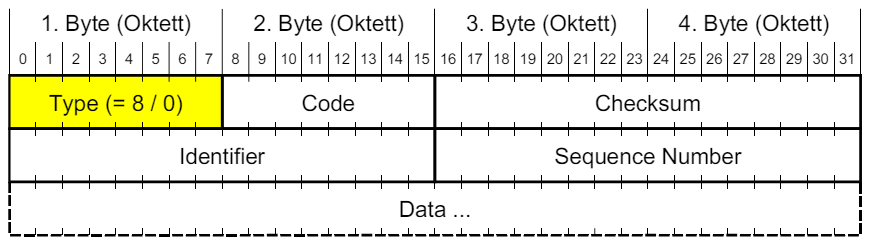
\includegraphics[width=0.75\linewidth]{images/icmp_echorequest.png}\\
    \textbf{ping} verwendet Echo und Echo Reply, um die Erreichbarkeit eines Routers/Hosts zu prüfen; ebenfalls wird die Round-Trip Zeit gemessen\\
        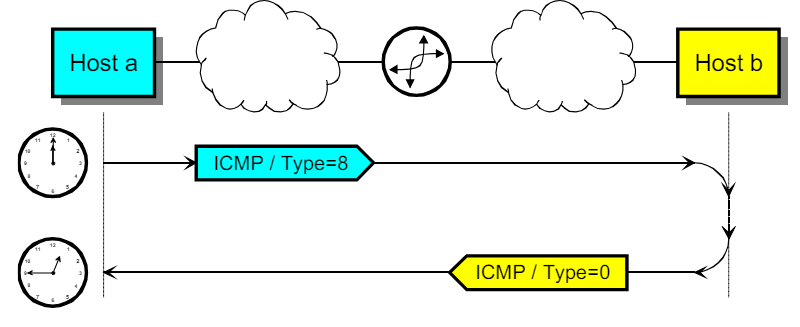
\includegraphics[width=0.75\linewidth]{images/ping.png}
\end{definition}

\begin{definition}{ICMP Destination Unreachable}\\
    Vom Router/Zielhost an Absender gesendet, wenn Paket nicht weitergeleitet werden kann\\
        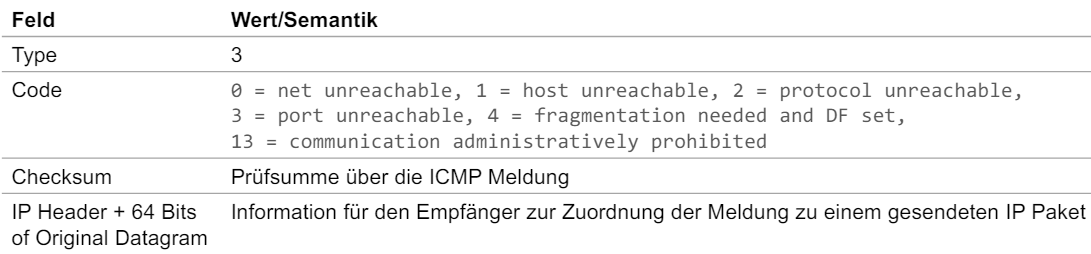
\includegraphics[width=1\linewidth]{images/destination_unreachable.png}\\
    \textbf{Path MTU Discovery:}\\
    Ziel
    \begin{itemize}
        \item Erkennung der kleinsten MTU auf Pfad zwischen Sender und Empfänger (Path-MTU, PMTU)
        \item RFC 1191 → Path MTU discovery
    \end{itemize}
    Zweck
    \begin{itemize}
        \item Vermeidung von Fragmentierung «unterwegs»
    \end{itemize}
\end{definition}

\begin{example}
        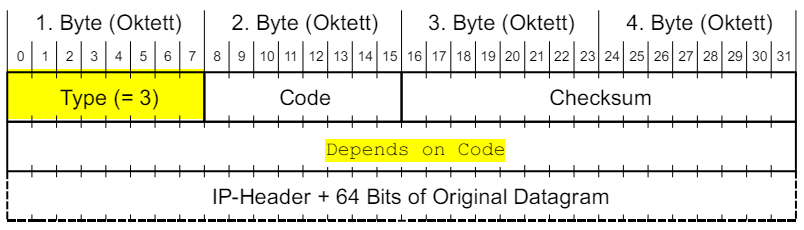
\includegraphics[width=0.75\linewidth]{images/dest_unreachable_ex1.png}\\
    Welche Codes werden von einem Router (0,1,4) und welche vom Zielhost (2,3) generiert?
    Welche vermutlich von einer Firewall (13)?
\end{example}

\begin{KR}{Path MTU discovery}\\
    Annahme, dass die PMTU gleich der lokalen MTU ist
    \begin{itemize}
        \item Senden von IP-Paketen mit Länge=PMTU und mit DF=1
        \item Empfang von «Destination Unreachable» mit Code 4 «fragmentation needed and DF set»
        \item PMTU reduzieren auf «Next-Hop MTU»
    \end{itemize}
    Die «Next-Hop MTU» erkennt man: Enthalten in Octet 5..8 («must be zero» stimmt nur, wenn wirklich «unused»)
\end{KR}

\begin{example2}{ICMP Destination Unreachable}\\
    Host 160.85.31.3 versucht, das folgende Paket an Host 160.85.29.99 zu senden (Farben siehe IP-Header def.):
    \begin{itemize}
        \item \textcolor{blue}{4500 0028} \textcolor{yellow}{8b10 0000} \textcolor{green}{0711} \textcolor{purple}{a8a4 \colorbox{lightgrey}{a055 1f03} \colorbox{lightgrey}{a055 1d63} 8b0d 829d 0014 a348 030a 0000 7504 1137 407c 0800}
        \item Erkennen Sie in diesem Paket die IP Adressen von Sender und Destination?
        \begin{itemize}
            \item \colorbox{lightgrey}{Sender}: a055 1f03, \colorbox{lightgrey}{Destination}: a055 1d63
        \end{itemize}
    \end{itemize}
    Ein Router kennt keinen Weg und sendet diese Destination Unreachable Message zurück (Farben siehe ICMP-Header def):
    \begin{itemize}
        \item 4500 0038 8038 0000 fd\textbf{01} 5bc0 \colorbox{lightgrey}{a055 821e a055 1f03} \textcolor{blue}{03}\textcolor{green}{01 4bf7} \textcolor{pink}{0000 0000} \textcolor{purple}{4500 0028 8b10 0000 0711 a8a4 a055 1f03 a055 1d63 8b0d 829d 0014 a348}
        \item Wie erkennen Sie, dass es sich um eine ICMP Message handelt? \textbf{Protocol}: 01
        \item Wie erkennen Sie den ICMP Typ? \textcolor{blue}{Type}: 03
        \item Erkennen Sie die "64 Bytes of Original Datagram"? \textcolor{purple}{Original Data}
    \end{itemize}
\end{example2}

\begin{definition}{ICMP Time Exceeded}
    \begin{itemize}
        \item \textcolor{blue}{Type = 11}
        \item \textcolor{pink}{unused (must be 0)}
    \end{itemize}
    Wird in diesen 2 Fällen gesendet:
    \begin{itemize}
        \item Router setzt TTL-Feld von 1 auf 0
        \begin{itemize}
            \item Paket wird verworfen und der Absender informiert (Code = 0)
        \end{itemize}
        \item Zielhost kann ein fragmentiertes Paket nicht innerhalb nützlicher Zeit reassemblieren
        \begin{itemize}
            \item Fragmente werden verworfen und der Absender informiert (Code = 1)
        \end{itemize}
    \end{itemize}
    \textbf{traceroute} erlaubt, den Weg zu einem beliebigen Host (oder einem fehlerhaft konfigurierten Router auf diesem Weg) zu finden
    \begin{itemize}
        \item UDP Datagramme an hohe Destination Portnummer (zufällig gewählt, default 33434)
        \item Erstes Datagramm: TTL := 1
        \begin{itemize}
            \item Erster Router setzt TTL auf 0, verwirft Paket und sendet Time Exceeded Message zurück
            \item Erste Router ist bekannt
        \end{itemize}
        \item Nächstes Datagramm: TTL := 2
        \begin{itemize}
            \item Zweiter Router ist bekannt etc...
        \end{itemize}
        \item …
        \item Zielhost kann Zielport nicht erreichen
        \begin{itemize}
            \item Destination Unreachable Message (Code = 1) an Absender
            \item Zielhost ist erreicht
        \end{itemize}
        \item Um die "Entfernung" zu den einzelnen Routern/Zielhosts zu bestimmen, wird zugleich noch die Round-Trip Zeit gemessen
    \end{itemize}
        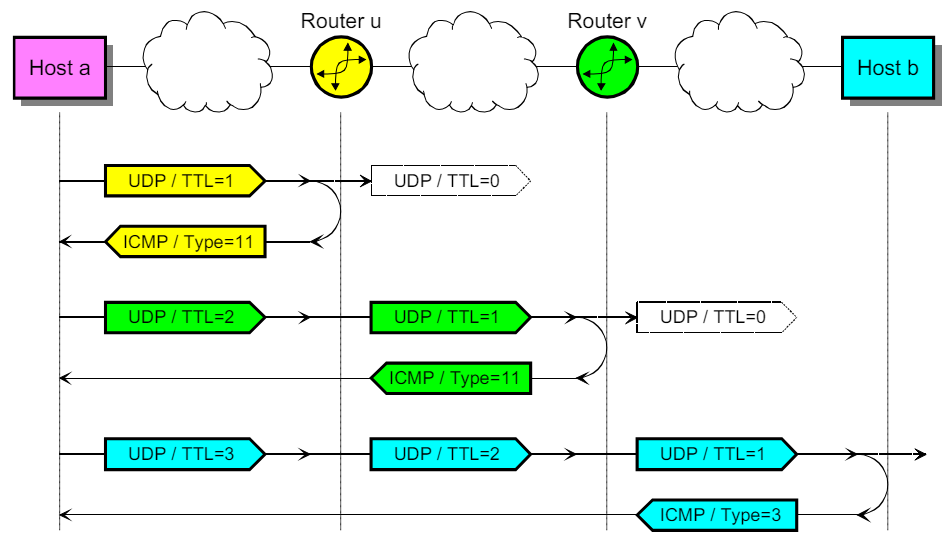
\includegraphics[width=1\linewidth]{images/traceroute.png}
\end{definition}











